% This file was created with matplot2tikz v0.5.3.
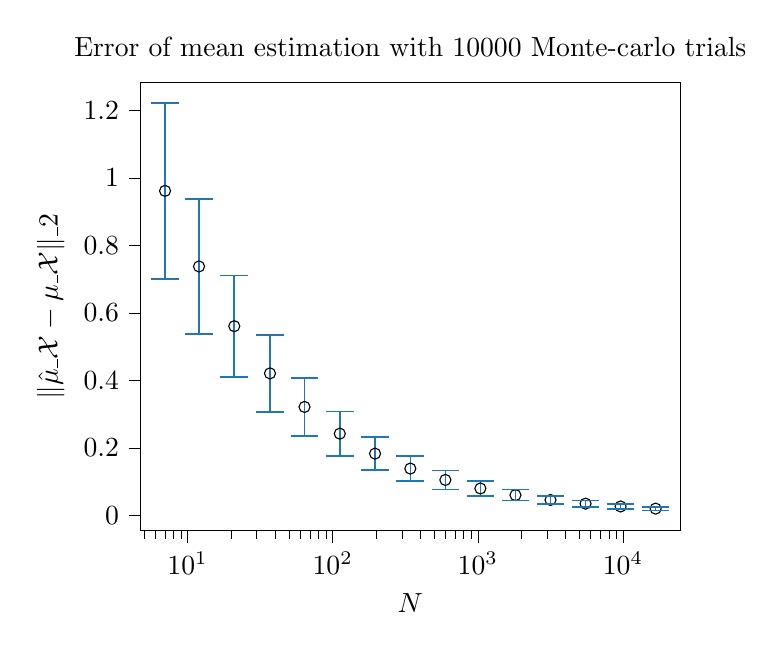
\begin{tikzpicture}

\definecolor{darkgray176}{RGB}{176,176,176}
\definecolor{steelblue31119180}{RGB}{31,119,180}

\begin{axis}[
log basis x={10},
tick align=outside,
tick pos=left,
title={Error of mean estimation with 10000 Monte-carlo trials},
x grid style={darkgray176},
xlabel={\(\displaystyle N\)},
xmin=4.74327639380337, xmax=24803.3195269196,
xmode=log,
xtick style={color=black},
y grid style={darkgray176},
ylabel={\(\displaystyle \|\hat{\boldsymbol{\mu}}\_\mathcal{X} - \boldsymbol{\mu}\_\mathcal{X}\|\_2\)},
ymin=-0.0461003164651899, ymax=1.28319327993008,
ytick style={color=black}
]
\addplot [draw=black, mark=o, only marks]
table{%
x  y
7 0.961809938446161
12 0.737728543463078
21 0.560616951169621
37 0.420661897373797
64 0.32120978405099
112 0.242018240638433
196 0.182805838986852
343 0.138405338128785
598 0.104765688177838
1042 0.0794917535174116
1818 0.0598006596884444
3170 0.0453866342512824
5528 0.0343647504602777
9639 0.026099922904704
16807 0.0196559171311048
};
\path [draw=steelblue31119180, semithick]
(axis cs:7,0.700849033162032)
--(axis cs:7,1.22277084373029);

\path [draw=steelblue31119180, semithick]
(axis cs:12,0.537975705847932)
--(axis cs:12,0.937481381078224);

\path [draw=steelblue31119180, semithick]
(axis cs:21,0.409881143046451)
--(axis cs:21,0.711352759292791);

\path [draw=steelblue31119180, semithick]
(axis cs:37,0.306090426059901)
--(axis cs:37,0.535233368687693);

\path [draw=steelblue31119180, semithick]
(axis cs:64,0.234693244705277)
--(axis cs:64,0.407726323396703);

\path [draw=steelblue31119180, semithick]
(axis cs:112,0.176615269618465)
--(axis cs:112,0.307421211658401);

\path [draw=steelblue31119180, semithick]
(axis cs:196,0.133295627068537)
--(axis cs:196,0.232316050905168);

\path [draw=steelblue31119180, semithick]
(axis cs:343,0.101071846947206)
--(axis cs:343,0.175738829310364);

\path [draw=steelblue31119180, semithick]
(axis cs:598,0.0764314707238397)
--(axis cs:598,0.133099905631837);

\path [draw=steelblue31119180, semithick]
(axis cs:1042,0.0578812731877006)
--(axis cs:1042,0.101102233847123);

\path [draw=steelblue31119180, semithick]
(axis cs:1818,0.0435629040530663)
--(axis cs:1818,0.0760384153238226);

\path [draw=steelblue31119180, semithick]
(axis cs:3170,0.0331333015828912)
--(axis cs:3170,0.0576399669196737);

\path [draw=steelblue31119180, semithick]
(axis cs:5528,0.0251640440466649)
--(axis cs:5528,0.0435654568738906);

\path [draw=steelblue31119180, semithick]
(axis cs:9639,0.0190071644585281)
--(axis cs:9639,0.0331926813508799);

\path [draw=steelblue31119180, semithick]
(axis cs:16807,0.0143221197345949)
--(axis cs:16807,0.0249897145276147);

\addplot [semithick, steelblue31119180, mark=-, mark size=5, mark options={solid}, only marks]
table {%
7 0.700849033162032
12 0.537975705847932
21 0.409881143046451
37 0.306090426059901
64 0.234693244705277
112 0.176615269618465
196 0.133295627068537
343 0.101071846947206
598 0.0764314707238397
1042 0.0578812731877006
1818 0.0435629040530663
3170 0.0331333015828912
5528 0.0251640440466649
9639 0.0190071644585281
16807 0.0143221197345949
};
\addplot [semithick, steelblue31119180, mark=-, mark size=5, mark options={solid}, only marks]
table {%
7 1.22277084373029
12 0.937481381078224
21 0.711352759292791
37 0.535233368687693
64 0.407726323396703
112 0.307421211658401
196 0.232316050905168
343 0.175738829310364
598 0.133099905631837
1042 0.101102233847123
1818 0.0760384153238226
3170 0.0576399669196737
5528 0.0435654568738906
9639 0.0331926813508799
16807 0.0249897145276147
};
\end{axis}

\end{tikzpicture}
